\section{Motivación}

\begin{frame}
	\frametitle{\secname}
	\begin{columns}
		\begin{column}{.48\paperwidth}
			\begin{alertblock}{¿Por qué el método de los volúmenes finitos?}
				\begin{enumerate}
					\item

					      Se obtiene un {\usebeamercolor[fg]{structure} esquema
							      conservativo} al
					      discretizar~\eqref{eq:conservationlaw} desde su forma integral.
					      \begin{equation}\label{eq:conservationlaw}
						      \diffp{U}{t}+
						      \diffp{f\left(U\right)}{x}=
						      0.
					      \end{equation}

					      \

					\item

					      Los esquemas lineales de diferencias finitas con
					      orden de convergencia mayor o igual que $2$ son
					      inestables para~\eqref{eq:conservationlaw}
					      ({\usebeamercolor[fg]{structure} Teorema de la
						      Barrera de orden de Godunov}~\cite{Godunov1959}).

					      \

					\item

					      El método de Galerkin conforme genera
						      {\usebeamercolor[fg]{structure} oscilaciones
							      espurias} en problemas hiperbólicos.
					      Se requieren técnicas adicionales Galerkin
					      Discontinuo o método estabilizados como Streamline
					      Upwind Petrov-Galerkin, mientras que FVM maneja
					      discontinuidades.
				\end{enumerate}
			\end{alertblock}
		\end{column}
		\begin{column}{.48\paperwidth}
			\begin{figure}[ht!]
				\centering
				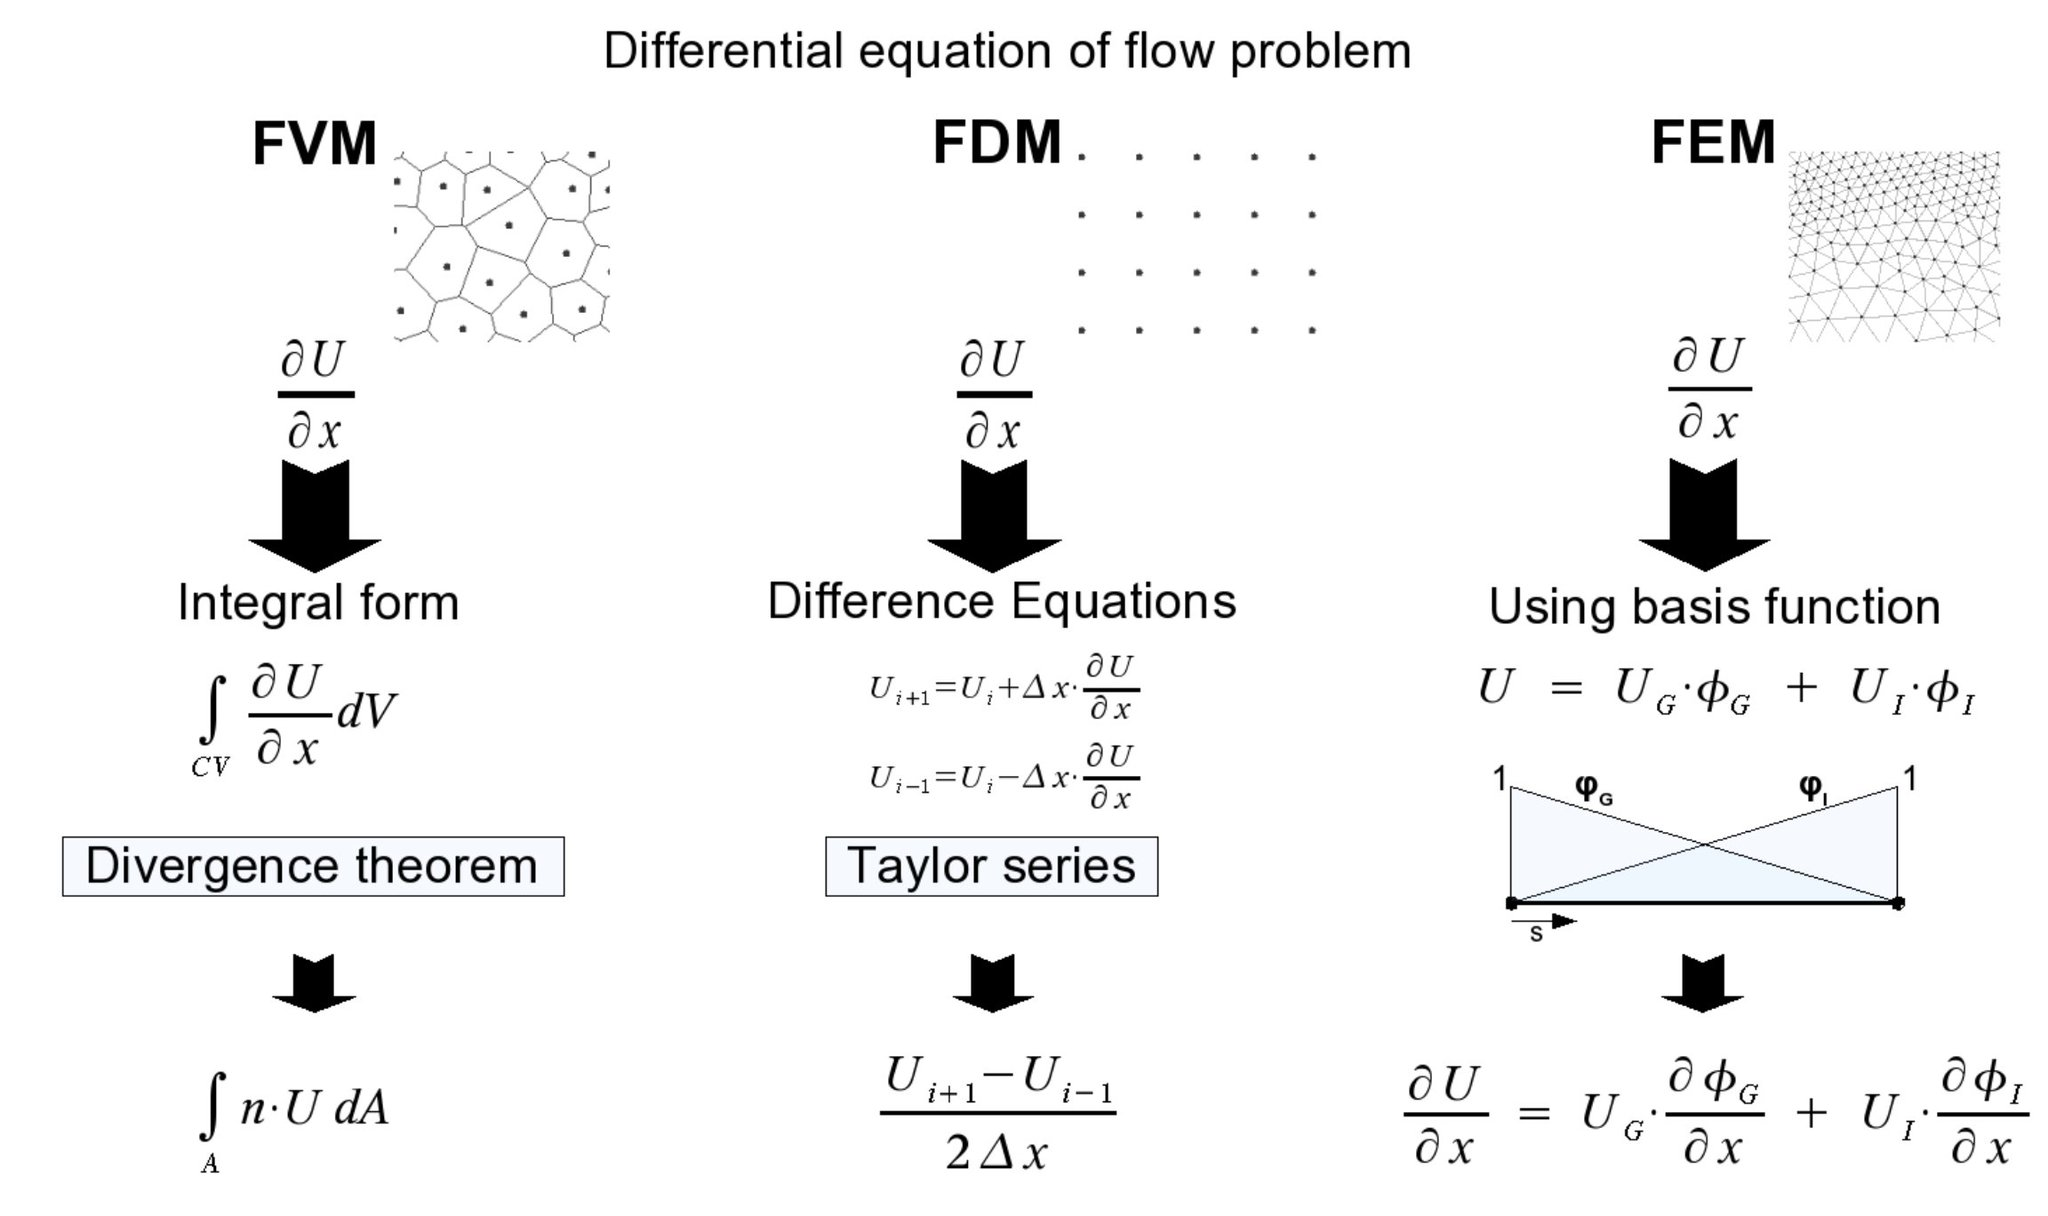
\includegraphics[width=.45\paperwidth]{methods.pdf}
				\caption{Comparativa de los métodos de discretización
					para~\eqref{eq:conservationlaw}~\cite{Milbradt2008}.}
			\end{figure}
		\end{column}
	\end{columns}
\end{frame}
